\chapter{Resultados}

En este capítulo pasamos a explicar cada experimento realizado, las métricas que se usarán para medir los resultados y haremos una serie de comentarios al respecto.
%TODO_DONE: introduce lo que se va a hacer en este capítulo

\section{Métricas}

Antes de pasar a mostrar los experimentos realizados vamos a explicar en qué consisten las dos métricas en las que nos basaremos para cotejarlos: el \ac{mIoU} y el \ac{MAE}.

\subsection{mIoU}

Para saber qué porcentaje de acierto ha tenido el proceso de segmentación semántica utilizaremos la métrica conocida como \ac{mIoU} \cite{miou-iou}. Esta métrica se basa en hacer la media de la \ac{IoU} de las diferentes etiquetas de clases.

La \ac{IoU} \cite{miou-iou} es la relación de superposición que existe entre la imagen segmentada y la original. Es decir, sirve para dictaminar con cuánta precisión se ha realizado el proceso de \ac{SS}. En las siguientes figuras se puede ver un ejemplo muy práctico:

\begin{figure}[H]
  \centering
  \includegraphics[width=8cm]{Figuras/Iou_1.eps}
  \caption{Imagen Original}
\end{figure}

\begin{figure}[H]
  \centering
  \includegraphics[width=8cm]{Figuras/IoU_2.eps}
  \caption{Predicción}
\end{figure}

\subsection{MAE}

Con el objetivo de evaluar con cuánta precisión se ha estimado la velocidad, vamos a servirnos de la métrica más adecuada para ello: el \ac{MAE} \cite{mae}. Ésta se basa en calcular la media de la diferencia absoluta de los valores reales con los valores de predicción de la velocidad. Como se puede ver en la fórmula \ref{eq:mae}, \textit{X} es una matriz con los valores reales e \textit{Y} es una matriz con los valores de predicción.

\begin{equation}\label{eq:mae}
MAE = \frac{\sum_{i=1}^{n}|X_i - Y_i|}{n}
\end{equation}

Con ello lo que conseguimos es saber de forma precisa el porcentaje de error que ha tenido la estimación en comparación con el valor real. Cuanto más bajo sea el \ac{MAE}, más veraz será la estimación.
%TODO_DONE: yo suelo añadir una sección explicando las métricas, pero no es necesario, si las explicas en cada experimento. Recuerda traer aquí la explicación de la mIOU para evaluar la segmentación semántica.

%TODO_DONE: organiza en secciones los distintos experimentos.
\section{Evaluación de la segmentación semántica}

Previo a mostrar los resultados finales del sistema $ISA^{2}$, vamos a ver qué resultados hemos obtenido en Swiftnet tanto para Cityscapes como para la base de datos de $ISA^{2}$.

\subsection{Swiftnet con Cityscapes}

Si se han seguido las indicaciones del capítulo anterior, tras ejecutar el modelo obtendremos el resultado de la figura \ref{fig:Res_Swift} en la terminal del sistema operativo:

\begin{figure}[H]
\centering
\includegraphics[width=12cm]{Figuras/Res_Swiftnet_Cityscapes.eps}
\caption{Resultados del modelo Swiftnet con base de datos Cityscapes}
\label{fig:Res_Swift}
\end{figure}

Como se puede ver, el resultado es el mismo que aparece en el paper de Swiftnet (75.52\% de \ac{mIoU}) junto a diferentes resultados de \ac{IoU} para cada una de las clases detectadas \cite{swiftnet}. A continuación, y para aclarar los resultados de forma visual, mostramos una comparativa de una imagen real y otra segmentada de Cityscapes:

\begin{figure}[H]
\centering
  \begin{subfigure}[b]{0.45\linewidth}
    \includegraphics[width=\linewidth]{Figuras/Imagen_Cityscapes_Real.eps}
    \caption{Imagen real de Cityscapes}
  \end{subfigure}
    \begin{subfigure}[b]{0.45\linewidth}
    \includegraphics[width=\linewidth]{Figuras/Imagen_Cityscapes_Segmentada.eps}
    \caption{Imagen segmentada de Cityscapes}
  \end{subfigure}
  \caption{Resultados de Swiftnet con Cityscapes}
\end{figure}

Como se puede apreciar (a simple vista), la segmentación ha sido correcta y el modelo ha sabido distinguir cada clase de la imagen con gran exactitud. En conclusión, la ejecución de Swiftnet ha sido un éxito.

\subsection{Swiftnet con $ISA^{2}$}

Para esta parte no contaremos con las métricas de \ac{mIoU} anteriores ya que la base de datos de $ISA^{2}$ no tiene máscaras de segmentación como Cityscapes, por lo que no se puede saber con cuánta precisión se van a segmentar las imágenes más que por los resultados de Cityscapes (que son los mismos que vienen en el paper de Swiftnet \cite{swiftnet}). De este modo, sólo mostraremos la comparativa entre una imagen real de esta base de datos junto con la imagen segmentada de la misma:

\begin{figure}[H]
\centering
  \begin{subfigure}[b]{0.45\linewidth}
    \includegraphics[width=\linewidth]{Figuras/Imagen_ISA2_Real.eps}
    \caption{Imagen real de $ISA^{2}$}
  \end{subfigure}
    \begin{subfigure}[b]{0.45\linewidth}
    
\includegraphics[width=\linewidth]{Figuras/Imagen_ISA2_Segmentada.eps}
    \caption{Imagen segmentada de $ISA^{2}$}
  \end{subfigure}
  \caption{Resultados de Swiftnet con $ISA^{2}$}
\end{figure}

\section{Evaluación del sistema $ISA^{2}$}

A continuación vamos a desarrollar cómo se realizará esta evaluación de la velocidad según la base de datos de $ISA^{2}$. Explicaremos cómo se realiza tanto para Swiftnet como para DeepLab y, tras obtener los resultados, detallaremos por qué son de esa forma, es decir, qué ha influido en ellos para que sean así; finalmente, comentaremos qué sistema de regresión da mejores resultados de entre todos ellos. Para ello nos serviremos de la métrica \ac{MAE} anteriormente nombrada.

Cabe destacar que Swiftnet \cite{swiftnet} es un modelo \textbf{Real-Time}, de modo que su implementación es menos que costosa que DeepLab, el cual, por el contrario, necesita de un tiempo de procesamiento demasiado elevado para realizar su función. En concreto Swiftnet trabaja a 39.9 \ac{FPS} para la resolución de Cityscapes (\textbf{1024 x 2048}) usando una tarjeta gráfica \textbf{NVIDIA GTX 1080 Ti} (la nuestra), mientras que DeepLab trabaja a 8 \ac{FPS} en una \textbf{NVIDIA Titan X} \cite{deeplab}; esta última tiene características que, en comparación con la nuestra, hacen que sea una tarjeta gráfica con un rendimiento sensiblemente peor \cite{gtx_titan}. Como resultado se puede ver que la diferencia del tiempo de procesado entre ambos modelos es notable, a pesar de trabajar sobre dos tarjetas gráficas con distintas características; ya que la diferencia entre ambas, aunque latente, \textcolor{Red}{no influye en gran medida para medir estos tiempos}. %TODO_DONE: añade información de tiempos de procesado de uno y otro, en lo que se refiere a segmentación semántica.

\subsection{Diseño del experimento}

Para realizar la evaluación de la velocidad en $ISA^{2}$ vamos a trabajar de la siguiente forma. Los sistemas de regresión funcionan de manera que necesitan de cierta información para poder ser entrenados y, después, poder predecir (en base a ese entrenamiento) los resultados que se esperan de ellos. Parte de dicha información se compone de la base de datos de $ISA^{2}$, de la cual pasamos a explicar cómo está organizada y cómo se utilizará en esta parte del proyecto.

En el capítulo \ref{ch:isa2} explicábamos que la base de datos de $ISA^{2}$ estaba compuesta por dos carpetas (\textbf{Highway} y \textbf{Urban}) correspondientes a imágenes en autovías y entornos urbanos. Internamente, estaban organizadas por subcarpetas que contenían las imágenes que se usarían para realizar los experimentos (\textbf{H1} y \textbf{H2} para \textit{Highway}, y \textbf{U1}, \textbf{U2} y \textbf{U3} para \textit{Urban}). Para este experimento usaremos el mismo sistema de directorios con la diferencia de que, en esta ocasión, las imágenes habrán sido procesadas por el modelo Swiftnet, y no por DeepLab.

Los sistemas de regresión funcionan de manera que necesitan de cierta información para poder ser entrenados y, después, poder predecir (en base a ese entrenamiento) los resultados que se esperan de ellos.

Para entrenar los sistemas usaremos las funciones de MatLab que explicábamos en el capítulo anterior. Sin embargo, el parámetro \textit{X}, común a dichas funciones, no representará a un sólo descriptor de imagen, sino a todo un set de éstos correspondientes a las imágenes de una de las subcarpetas antes mencionadas. Lo mismo pasa con el parámetro \textit{Y}: Éste tendrá información de la velocidad adecuada para cada una de las imágenes de dicha subcarpeta; esta información la tenemos guardada en unos archivos ``.mat''.

Dicho esto pasamos a señalar con qué subcarpetas entrenamos el modelo, o dicho de otra forma, qué contendrá el parámetro \textit{X}: Para el caso de las autovías lo haremos con la subcarpeta \textbf{H2}, y para los entornos urbanos usaremos las subcarpetas \textbf{U1} y \textbf{U2}.

Ya hemos hablado acerca de cómo se entrenan los sistemas de regresión y con qué secuencias de imágenes se hace. Ahora pasamos a explicar cómo se realiza la predicción.

Para que los sistemas puedan predecir estimaciones de la velocidad nos serviremos de una función de MatLab llamada:

\begin{center}
\textit{predict(Mdl,Z)}
\end{center}

Esta función (\cite{predict}) devuelve como respuesta la predicción del modelo de regresión lineal \textit{Mdl} para los datos de prueba de la matriz \textit{Z}. Los datos de prueba de dicha matriz se corresponderán con una subcarpeta del anterior sistema de archivos. Para las autovías escogeremos la subcarpeta \textbf{H1}, mientras que para los entornos urbanos escogeremos \textbf{U3}.

Cabe destacar que esta función se utiliza en 3 de los 4 sistemas de regresión que hemos utilizado, puesto que en Lasso predecimos los resultados limitando el tamaño de los coeficientes de regresión \cite{coef_lasso}.
%TODO_DONE hay que añadir una subsección donde se explique el diseño del experimento, es decir, qué se emplea para training, y qué para test, de cada una de las secuencias que forman ISA^2

En la siguiente tabla pasamos a mostrar los resultados tanto de la versión anterior de $ISA^{2}$ \cite{isa2} como de la desarrollada en este trabajo. Como ya dijimos anteriormente, el \ac{MAE} será la métrica que usaremos para esta tarea, pues indica cuánta precisión ha habido en términos de la estimación de la velocidad.

\begin{table}[H]
\centering
\resizebox{16cm}{!}{
\begin{tabular}{|l|l|l|l|l|l|}\cline{1-6}
& & \multicolumn{2}{|l|}{\textbf{MAE Swiftnet}} & \multicolumn{2}{|l|}{\textbf{MAE DeepLab}} \\ \cline{1-6}
\textbf{Regresión} & \textbf{Nivel de \ac{SPP}} & \textbf{Highway (\%)} & \textbf{Urban (\%)} & \textbf{Highway (\%)} & \textbf{Urban (\%)}\\ \cline{1-6}
\multirow{4}{*}{\textbf{\textit{Lineal}}} & 1 & 12.22 & 8.95 & 10.32 & 8.38 \\ \cline{2-6}
& 2 & 13.94 & 9.45 & 11.18 & 8.81 \\ \cline{2-6}
& 3 & 13.39 & \textbf{\textit{11.79}} & 15.5 & \textbf{\textit{10.83}}\\ \cline{2-6}
& 4 & \textbf{\textit{55.61}} & \textbf{\textit{12.19}} & \textbf{\textit{55.61}} & \textbf{\textit{12.19}} \\ \cline{1-6}
\multirow{4}{*}{\textbf{\textit{Lasso}}} & 1 & 12.90 & 9.23 & 11.29 & 8.43 \\ \cline{2-6}
 & 2 & 13.80 & 9.40 & 11.7 & 8.62 \\ \cline{2-6}
 & 3 & 13.47 & 10.16 & 10.8 & 9.25\\ \cline{2-6}
 & 4 & 13.7 & 9.63 & 13.7 & 9.42\\ \cline{1-6}
\multirow{4}{*}{\textbf{\textit{Boosting Trees}}} & 1 & 13.43 & \textbf{9.83} & 11.35 & \textbf{10.14} \\ \cline{2-6}
 & 2 & 14.97 & \textbf{10.52} & 12.23 & \textbf{10.72}\\ \cline{2-6}
 & 3 & 14.75 & \textbf{10.08} & 10.37 & \textbf{10.12}\\ \cline{2-6}
 & 4 & \textbf{14.16} & \textbf{10.02} & \textbf{14.22} & \textbf{10.02}\\ \cline{1-6}
\multirow{4}{*}{\textbf{\textit{SVR}}} & 1 & 11.13 & \textbf{8.74} & 9.69 & \textbf{9.55} \\ \cline{2-6}
 & 2 & 12.24 & \textbf{8.98} & 9.98 & \textbf{9.09}\\ \cline{2-6}
 & 3 & 12.09 & \textbf{9.60} & 9.78 & \textbf{9.62}\\ \cline{2-6} 
 & 4 & \textbf{12.01} & 9.53 & \textbf{12.08} & 9.52\\ \cline{1-6}
\end{tabular}
}
\caption{Tabla de resultados} %TODO_DONE: añade más información , sobre qué experimento, incluso comenta el ganador.
\label{tab:Resul_ISA2}
\end{table}

Los valores de Swiftnet que aparecen \textbf{resaltados} indican que son mejores que los valores de DeepLab (\textbf{también resaltados}) para esa fila.

Estos resultados se han generado siguiendo el proceso de entrenamiento y prueba anteriormente indicado en cada uno de los sistemas, es decir: utilizando las subcarpetas \textbf{H2}, \textbf{U1} y \textbf{U2} para entrenar los sistemas, siendo la primera la correspondiente a autovías y el resto a escenarios urbanos; y usando las subcarpetas \textbf{H1} (autovías) y \textbf{U3} (núcleos urbanos) como prueba.

Como se puede apreciar para este experimento, los mejores resultados son los que da el sistema \textit{\ac{SVR}} en todos los niveles de agrupación para entornos urbanos (con la excepción del nivel 4 que, en autovías, es sensiblemente mejor usando Swiftnet, y en entornos urbanos el \ac{MAE} de ambos modelos está casi a la par). El sistema \textit{Boosting Trees} tampoco se queda atrás y en todos sus niveles consigue lo mismo que el sistema \ac{SVR}: Una mejora del \ac{MAE} de Swiftnet con respecto del de DeepLab en entornos urbanos y, en el último nivel, volviendo a tener dicha mejora en autovías. El resto de sistemas (\textit{Lasso y Lineal} siguen siendo peores ejecutándose con los resultados de Swiftnet, y en concreto el sistema de regresión \textit{Lineal}, para el nivel de agrupación 4, es el que da unos resultados realmente catastróficos a pesar de haber sido corregidos como explicamos más adelante.%TODO_DONE: da más detalles, donde se entrena, dódne se prueba, se trata de repetir lo del diseño del experimento

Es en este punto en que el que se puede ver la influencia que tiene \ac{SPP} sobre los descriptores de imagen y, por lo tanto, sobre los resultados de la tabla. 

Cuando generamos los descriptores de imagen estamos utilizando \ac{SPP} para que, según el nivel de agrupación que se use, se obtenga más o menos información en éstos. Recordemos que el nivel de agrupación indica el nivel de granularidad que tendrán los descriptores, y por lo tanto la cantidad de información que llevarán consigo.

Analizando la tabla \ref{tab:Resul_ISA2}, vemos cómo para mayores niveles de agrupación, la precisión de los sistemas de regresión va en aumento. Esto puede verse en los niveles 3 y 4 de todos los sistemas, exceptuando el \textit{Lineal} que de ahora en adelante excluiremos por la poca certeza de sus resultados en comparación con el resto. Entre estos niveles, la diferencia entre el \ac{MAE} de un modelo en un determinado escenario con el \ac{MAE} del mismo modelo en el mismo escenario (pero en un distinto nivel) es muy pequeña. Esto es porque cuando aumentamos al nivel 4, el grado de granularidad es superior y tendrá más precisión para estimar la velocidad en comparación con el anterior, sin embargo, el nivel 3 también aporta una granularidad muy alta y, por ende, una estimación muy precisa; por lo tanto, si con el nivel 3 ya obtenemos resultados concisos, con el nivel 4 podemos refinarlos hasta obtener una estimación con mayor nivel de certeza.

\textcolor{Red}{Esto no siempre es así, porque puede pasar que en el nivel 4 se tomen en consideración datos que el nivel 3 había pasado por alto y como resultado nos dé un \ac{MAE} mayor en el último nivel. A lo que nos referimos con todo esto es a la posibilidad de que mientras los sistemas de regresión se ejecutan con datos de nivel 3, al no tener la misma profundidad que los de nivel 4, puedan obviar información relevante que con un nivel superior serían capaces de procesar. Esto se puede ver, por ejemplo, en la estimación del sistema \textit{Lasso} tanto para Swiftnet como para DeepLab. Sin embargo, este suceso no ocurre sólo en los niveles 3 y 4, para comprobarlo basta con revisar los niveles iniciales del sistema \textit{\ac{SVR}}}.

Dicho todo esto, y comparando los valores de la tabla, podemos asegurar que los mejores sistemas con Swiftnet son \textit{Boosting Trees} y \textit{\ac{SVR}}. Para concretar más, vamos a puntualizar cómo el sistema \textit{\ac{SVR}} es mejor incluso, y es debido al reducido \ac{MAE} que tiene en todos sus niveles en comparación con el sistema \textit{Boosting Trees}.

En conclusión, podemos afirmar que el mejor sistema de regresión que se puede utilizar para el modelo Swiftnet es \textit{\ac{SVR}}.

\subsection{Problema del sistema de regresión \textit{Lineal} y cómo aliviarlo}

Hemos puesto dos valores con \textit{\textbf{este aspecto}} para indicar que, durante la predicción de la velocidad en el sistema de regresión lineal, hemos modificado una función para obtener unos resultados más apropiados; ya que, de otra forma, se obtendrían valores muy lejanos de la realidad. Nos referimos a la función \textit{filter}:

\begin{center}
\textit{filter(B,1,YHat)}
\end{center}

Esta función filtra los datos de predicción de la matriz \textit{YHat} utilizando una función de transferencia racional definida por los coeficientes del numerador y del denominador \textit{B} y \textit{1} respectivamente, siendo \textit{B} una matriz \cite{filter}. Los coeficientes de esta matriz los generaremos de la siguiente forma:

\begin{center}
\textit{B = 1\textbackslash{n}*ones(n,1)}
\end{center}

Lo que hace la instrucción anterior es crear una matriz de unos (\textit{ones}) de \textit{n} filas y 1 columna, y multiplicar los valores por un factor de \textit{1\textbackslash{n}}. Este va a ser el punto en el que vamos a modificar el código para obtener resultados más acordes a lo que se espera, cambiando el valor de \textit{n} para que la función \textit{filter} filtre resultados que excedan por mucho la velocidad real.

Este problema sólo sucede en el sistema de regresión \textit{lineal}. Puede ser debido a que durante el proceso de \ac{SS} al aplicar niveles más altos de agrupación, se obtiene así más nivel de detalle en las imágenes, y por ende, en los descriptores de imagen; por lo que el sistema se confunde con la información de algunos de estos descriptores cuando están siendo entrenados o predichos, de tal modo que en ciertas partes de la regresión se obtienen picos de resultados que no se corresponden a la realidad. Esto puede ser ya que estos picos sólo suceden con niveles de agrupación mayores que 2, por lo que tiene sentido que se deba a algo así.

\begin{figure}[H]
\centering
  \begin{subfigure}[b]{0.45\linewidth}
    \includegraphics[width=\linewidth]{Figuras/Linear_Urban(Nivel_4)(Filter_1000000.eps}
    \caption{Lineal en entornos urbanos para \textbf{Nivel 4} con \textit{filter} a 1000000}
  \end{subfigure}
  \begin{subfigure}[b]{0.45\linewidth}
    \includegraphics[width=\linewidth]{Figuras/Linear_Highway(Nivel_4)(Filter_25000000.eps}
    \caption{Lineal en autovías para \textbf{Nivel 4} con \textit{filter} a 25000000}
  \end{subfigure}
  \caption{Resultados del sistema de regresión lineal modificando la función \textit{filter}}
\end{figure}

Con valores de \textit{n} de 400 en entornos urbanos y de 20 en autovías para nivel de agrupación 3 y de 10000000 en entornos urbanos y de 25000000 en autovías para nivel de agrupación 4 se puede llegar a aliviar el problema, pero indudablemente la predicción estará mal en comparación con los niveles anteriores.
%TODO_DONE Te refieres la filtrado? hay que explicarlo, dando detalles y poniendo las gráfica

%Como se puede observar, tanto los sistemas \textit{Boosting Trees} como \textit{\ac{SVR}} son mejores con la nueva versión de $ISA^2$ que integra Swiftnet para entornos urbanos, mientras que para las autovías es mejor utilizar el modelo DeepLab. Esto quiere decir que Swiftnet trabaja mejor con entornos en los que se requiere más nivel de detalle y DeepLab, por el contrario, lo realiza mejor en entornos más abiertos.

\subsection{Resultados finales}

A continuación mostramos algunas figuras con las que podemos ver, de forma gráfica, los resultados de los sistemas de regresión con la \ac{SS} realizada por Swiftnet:

\begin{figure}[H]
  \centering
  \begin{subfigure}[b]{0.45\linewidth}
    \includegraphics[width=\linewidth]{Figuras/Lineal_Highway(Nivel_1).eps}
    \caption{Highway con Lineal en nivel 1 de \ac{SPP}}
  \end{subfigure}
    \begin{subfigure}[b]{0.425\linewidth}
    \includegraphics[width=\linewidth]{Figuras/Lasso_Urban(Nivel_1).eps}
    \caption{Urban con Lasso en nivel 1 de \ac{SPP}}
  \end{subfigure}
    \begin{subfigure}[b]{0.45\linewidth}
    \includegraphics[width=\linewidth]{Figuras/Boosting_Urban(Nivel_1).eps}
    \caption{Urban con Boosting en nivel 1 de \ac{SPP}}
  \end{subfigure}
    \begin{subfigure}[b]{0.45\linewidth}
    \includegraphics[width=\linewidth]{Figuras/SVR_Urban(Nivel_1).eps}
    \caption{Urban con SVR en nivel 1 de \ac{SPP}}
  \end{subfigure}
  \caption{Resultados gráficos}
\end{figure}

En las figuras, los puntos azules representan la velocidad \textbf{real} a la que debe ir el vehículo en cada imagen, mientras que los puntos rojos representan la velocidad \textbf{estimada} por los sistemas de regresión en cada imagen.

Como se puede observar, hemos escogido, en su mayoría, aquellas figuras en las que los sistemas de regresión han dado mejores resultados, es decir, en entornos urbanos \textbf{(Urban)}. Sin embargo, para contrastar cómo trabaja Swiftnet en autovías hemos decidido poner una figura con esos datos (\textbf{Highway}). Nótese cómo hemos escogido los resultados con nivel de agrupación 1 en lugar de otros. Esto es porque, a pesar de que no tienen un gran nivel de detalle, son los que mejores resultados dan en comparación con los demás.

%TODO: faltan muchas cosas.
%TODO_DONE 1) Hay que aclarar que los anteriores resultados, para cada regresor, han sido obtenidos con unos parámetros para el spatial pyramids concretos. Debemos ponerlos.
%TODO_DONE: 2) Hay que enriquecer este capítulo con un análisis de la influencia del nivel de la pirámide para cada regresor, así se entenderá porqué hemos puesto los ganadores en la primera tabla. Básicamente una tabla donde comparemos todos con todos los niveles del 1 al 4.
%TODO_DONE: 3)falta una sección con los resultados de evaluación en cityscapes en términos de segmentación semántica, donde podamos ver que replicamos los resultados del paper original. Yo pondría esta subsección la primera.
%4) Resultados cualitativos: añadir imágenes donde se vea la predicción de la velocidad, y la velocidad anotada, hay que seleccionar las mejores y las peores, y comentarlo. Puedes hacerlo para el modelo ganador nuestro, y creas dos figuras, una con imágenes urbanas y otra con imágenes de autopista. Puedes poner las 4 mejores y las 4 peores. 
%5) Para el examen conviene que tengas una demo lista en la que podamos ver el sistema funcionando. Lo lanzas contra una carpeta de imágenes y va una a una generando la velocidad, que se guarda en una imagen donde se vea el dato superpuesto, como si fuera un video. Si tienes dudas comentamos. Eso te va a permitir generar un gif a modo de video que te va a quedar muy chulo. 
%TODO_DONE: 6) Hecho en falta un análsis tiempos de procesado del switnet, para terminar de vender lo de que es tiempo real, vaya. Debes añadirlo.
